\documentclass[eikonal.tex]{subfiles}

\begin{document}

\section{Classification of Ordered Line Integral Methods}

Each ordered line integral method (OLIM) corresponds to:
\begin{enumerate}
\item a means of selecting a neighborhood $n(\hat{p})$ of points for
  each grid point $\hat{p}$,
\item a method of exactly covering $\conv(n(\hat{p}))$ with a family
  of simplexes $\calC$,
\item algorithms for minimizing line integrals.
\end{enumerate}
The first two points are independent of the third. Algorithmically,
the first two points are concerned with how to iterate over the
simplexes in the decomposition of $\conv(n(\hat{p}))$. At the same
time, we can independently design algorithms for the third point by
minimizing line integrals on isolated simplexes. So, we can conceive
of generic ``neighborhood enumeration'' algorithms and line integral
minimization algorithms which can be combined in arbitrary ways.

Before looking at the line integral minimization algorithms, we will
describe the different ways we decompose $n(\hat{p})$. In two
dimensions, we have two methods: OLIM4 and OLIM8; in three, there are
three: OLIM6, OLIM18, and OLIM26. We will find that the trade-off
between these methods is between slowness and directional coverage
(accuracy).

In describing the various OLIMs, we will take $\hat{p} = 0$ without
loss of generality. We also assume that the simplexes in $\calC$
satisfiy the following definition.
\begin{defn}\label{def:olim-simplex}
  Let $C \in \calC$, let $v(C)$ denote the set of vertices of $C$, let
  $m$ be the ambient dimension, and let $m' = \dim(C) \leq m$. Then,
  if $\hat{p} \in v(C)$, and $p \in v(C) \backslash \set{\hat{p}}$
  implies $p \in n(\hat{p})$, call $C$ an \emph{OLIM simplex of
    dimension $m'$}.
\end{defn}
\noindent That is, each $C \in \calC$ is the convex hull of $\hat{p}$
and a dimension $\dim(C) - 1$ face of $\conv(n(\hat{p}))$.

Assuming $\hat{p} = 0$, this property lets us classify each simplex
$C \in \calC$ according to the Hamming weights of the vertices of $C$
in $n(\hat{p})$.
\begin{defn}
  Fix $\hat{p}$ and assume $\hat{p} = 0$. Let $C \in \calC$, and let
  $\set{p_0, \hdots, p_{m-1}} = v(C) \backslash \set{\hat{p}}$. Let
  $d_0 \leq \cdots \leq d_{m-1}$ denote the sorted Hamming weights of
  $p_0, \hdots, p_{m-1}$. Then, $(d_0, \hdots, d_{m-1})$ is the
  \emph{degree} of $C$.
\end{defn}
\noindent For $m = 2, 3$, we will drop the vector notation and abbreviate
$(d_0, d_1)$ and $(d_0, d_1, d_2)$ to $d_0d_1$ and $d_0d_1d_2$,
respectively.

\subsection{OLIM4 and OLIM8}

In this section, we will carefully walk through the choices that lead
to OLIM4 and OLIM8. In the next section, concering 3D OLIMs, we will
go more quickly and simply list important details.

Our naming convention for the different types of OLIM is to append the
cardinality of $n(\hat{p})$ to ``OLIM'': i.e. OLIM$k$ uses a $k$-point
stencil. To choose $n(\hat{p})$ (and hence $k$), we use the following
guidelines:
\begin{enumerate}
\item $n(\hat{p})$ should be symmetric about $\hat{p}$,
\item the only grid points contained in $\conv(n(\hat{p}))$ should be
  $\hat{p}$ and the points in $n(\hat{p})$,
\item $\conv(n(\hat{p}))$ should have maximum dimension.
\end{enumerate}
If we restrict ourselves to the eight nearest neighbors of $\hat{p}$,
these guidelines restrict us to two possible choices for
$n(\hat{p})$. Letting $e_i$ denote the standard basis vectors in
$\R^m$, we can choose:
\begin{align*}
  n(\hat{p}) = \set{\hat{p} \pm e_1, \hat{p} \pm e_2} \qquad \mbox{or} \qquad n(\hat{p}) = \set{\hat{p} \pm e_1, \hat{p} \pm e_2, \hat{p} \pm e_1 \pm e_2},
\end{align*}
where we range over all choices of sign. The first choice consists of
$k = 4$ points, and the second has $k = 8$.

With $n(\hat{p})$ selected, we can set about choosing $\calC$. To do
this, we construct $\calC$ as follows:
\begin{enumerate}
\item partition $\conv(n(\hat{p}))$ into a set of dimension $m$ OLIM
  simplexes such that the resultant set of simplexes is symmetric
  about $\hat{p}$---let $\calC$ initially equal this set,
\item for each pair $C, C' \in \calC$, if $C$ and $C'$ intersect, their intersection is a dimension $m - 1$ OLIM simplex---add these simplexes to $\calC$,
\item add OLIM simplexes of dimensions $m - 2, m - 3, \hdots, 1$ to
  $\calC$ by recursively applying the previous step.
\end{enumerate}
If we apply this procedure to the choice of
$n(\hat{p}) = \set{p_1, p_2, p_3, p_4}$ for OLIM4, we initially obtain
four triangles:
$\set{\hat{p}, p_1, p_2}, \set{\hat{p}, p_2, p_3}, \set{\hat{p}, p_3,
  p_4}, \set{\hat{p}, p_4, p_1}$. These triangles are all of dimension
$m = 2$, so we only look for dimension $m - 1 = 1$ OLIM simplexes
(lines) to add. We find $\set{\hat{p}, p_i}$ for $i = 1, 2, 3, 4$. The
procedure for OLIM8 is similar. For depictions of the resultant
stencils, see \cref{fig:olim4-stencil,fig:olim8-stencil}.

\begin{figure}
  \centering
  \begin{minipage}[c]{0.47\textwidth}
    \centering
    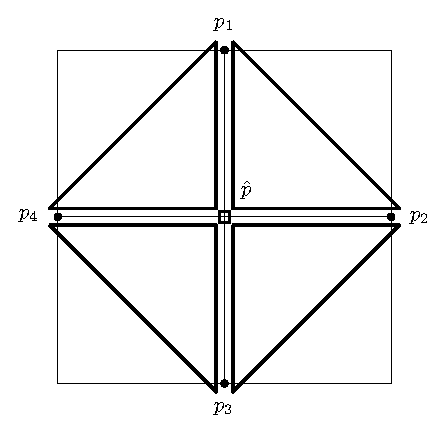
\includegraphics[width=\textwidth]{olim4-stencil.eps}
    \caption{the OLIM4 stencil, consisting of four degree (1, 1)
      triangular updates, and four degree 1 line updates. The
      triangular updates are shown using a slightly exploded diagram
      to ease visualization.}\label{fig:olim4-stencil}
  \end{minipage}
  \hfill
  \begin{minipage}[c]{0.47\textwidth}
    \centering
    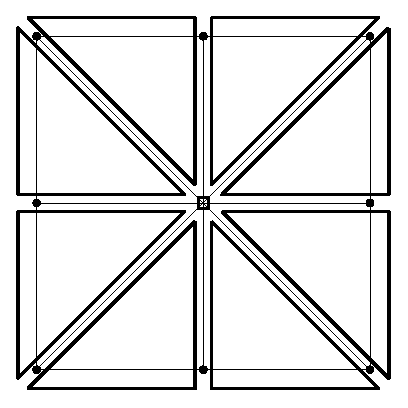
\includegraphics[width=0.9\textwidth]{olim8-stencil.eps}
    \caption{the stencil for the OLIM8 method, which consists of eight
      degree (1, 2) triangle updates, four degree 1 line updates, and
      four degree 2 line updates.}\label{fig:olim8-stencil}
  \end{minipage}
\end{figure}

\subsection{OLIM6, OLIM18, and OLIM26}

\section{The Update Algorithm}

With $\calC$ defined, our general update algorithm follows:

\begin{algorithm}[H]
  \caption{Compute $\hat{U} = U(\hat{p})$ (unconstrained version).}
  \begin{algorithmic}
    \FOR{$m' = 1, \hdots, m$}
      \FOR{$C \in \calC$ such that $\dim(C) = m'$}
        \IF{$\texttt{state}(p) = \texttt{valid}$ for all $p \in v(C) \backslash \set{\hat{p}}$}
          \STATE{} Let $\hat{U}_{\operatorname{new}}$ be the value of the minimized line integral.
          \STATE{} $\hat{U} \gets \min(\hat{U}, \hat{U}_{\operatorname{new}})$.
        \ENDIF{}
      \ENDFOR{}
    \ENDFOR{}
  \end{algorithmic}
\end{algorithm}

\end{document}

%%% Local Variables:
%%% mode: latex
%%% TeX-master: t
%%% End:
